\documentclass[11pt, a4paper]{article}

\usepackage{mlt-thesis-2015}

\usepackage[english]{babel}
\usepackage[hidelinks]{hyperref}
\usepackage{graphicx}
\usepackage{setspace}
\usepackage{comment}
\usepackage{caption}
\usepackage{listings}
\usepackage{textgreek}
\usepackage{lscape}
\usepackage{cancel}
\usepackage{amssymb}
\lstset{language=Python,basicstyle=\footnotesize,breaklines=true,breakatwhitespace=true,tabsize=4}

\usepackage[acronym]{glossaries}
\glsdisablehyper

\title{Implementing perceptual semantics in Type Theory with Records (TTR)}
%\subtitle{An implementation of visual perception and spatial relations in \gls{ttr}}
\author{Arild Matsson}
\date{}

\newacronym{hmm}{HMM}{Hidden Markov Model}
\newacronym{lstm}{LSTM}{Long Short-Term Memory}
\newacronym{cnn}{CNN}{convolutional neural network}
\newacronym{ttr}{TTR}{Type Theory with Records}
\newacronym{nlg}{NLG}{natural language generation}
\newacronym{vqa}{VQA}{visual question answering}
\newacronym{yolo}{YOLO}{You only look once}
\newacronym{nlp}{NLP}{natural language processing}
\newacronym{fol}{FOL}{first-order logic}
\newacronym{cfg}{CFG}{context-free grammar}

\newtheorem{definition}{Definition}

%\newcommand{\ttrmerge}{\mathrel{\substack{\wedge \\[-.3em] \cdot}}}
%\newcommand{\ttrmerge}{\mathrel{\underset\cdot\wedge}}
\newcommand{\ttrmerge}{\mathrel{\wedge_{\mkern-10mu\cdot\mkern6mu}}}
%\newcommand{\subtrlb}{\mathrel{\sqsubseteq\!\!\!\sqsubseteq}}
\newcommand{\subtrlb}{\mathrel{\sqsubseteq_\text{rlb}}}

\newcommand{\rec}[1]{\arraycolsep=.3em\left[\begin{array}{rcl}#1\end{array}\right]}



\begin{document}

%% ============================================================================
%% Title page
%% ============================================================================
\begin{titlepage}

\maketitle

\vfill

\begingroup
\renewcommand*{\arraystretch}{1.2}
\begin{tabular}{l@{\hskip 20mm}l}
\hline
Master's Thesis & 30 credits\\
Programme & Master’s Programme in Language Technology\\
Level & Advanced level \\
Semester and year & Spring, 2018\\
Supervisors & Simon Dobnik and Staffan Larsson \\
Examiner & Peter Ljunglöf \\
Keywords & type theory, image recognition, perceptual semantics, \\
& visual question answering, spatial relations, artificial intelligence
\end{tabular}
\endgroup

\thispagestyle{empty}
\end{titlepage}

%% ============================================================================
%% Abstract
%% ============================================================================
\newpage
\singlespacing
\glsresetall
\section*{Abstract}

\Gls{ttr} provides accounts of a wide range of semantic and linguistic phenomena in a single framework.
This work proposes a \gls{ttr} model of perception and language.
Utilizing PyTTR, a Python implementation of \gls{ttr}, the model is then implemented as an executable script.
Over pure Python programming, \gls{ttr} provides a transparent formal specification.
The implementation is evaluated in a basic \gls{vqa} use case scenario.
The results show that an implementation of a \gls{ttr} model can account for multi-modal knowledge representation and work in a \gls{vqa} setting.

% TTR also provides a connection between perception and a wide range of semantic phenomena described in TTR, e.g. quantification, inference, modality, negation, semantic coordination,.

\thispagestyle{empty}

%% ============================================================================
%% Preface
%% ============================================================================
\newpage
\section*{Acknowledgements}

Huge thanks to my supervisors and to professor Robin Cooper, all of whom have provided significant help through this process.

\thispagestyle{empty}

%% ============================================================================
%% Contents
%% ============================================================================
\newpage

\begin{spacing}{0.0}
\glsresetall
\tableofcontents
\end{spacing}

\thispagestyle{empty}

\newpage
\setcounter{page}{1}

\glsresetall
\section{Introduction}
\label{sec:intro}

Having computers understand visual input is desirable in several areas.
A domestic assistant robot may use a camera to navigate and identify useful objects in a home.
Driver-less cars need to be able to read road signs and track other moving vehicles.
Web crawlers may extract information from images alongside text on the web.

This kind of understanding involves processing sensory (such as visual) input on a cognitive level.
Low-level image processing may include tasks such as prominent color extraction, edge detection and visual pattern recognition.
Higher-level processing, however, includes identifying objects, their properties and their relations to each other.
This information can then be used for language understanding, reasoning, prediction and other cognitive processes.
Making the connection between sensory input and cognitive categories is what concerns the field of \textit{perceptual semantics} \citep{PustejovskyPerceptualsemanticsconstruction1990}.

Humans use language to communicate information.
Thus it is useful to add linguistic capacities to a perceptual system.
With vision and language connected, a robot can talk about what it sees, and descriptions can be automatically generated for images found on the web.
Image caption generation is indeed a popular task for evaluating computer vision systems.
Another one is \textit{\gls{vqa}} \citep{AgrawalVQAVisualQuestion2015}, where the system is expected to generate answers to natural-language questions in the context of a given image.

The connection between different modes of information, such as vision and language, requires a model of semantic representation.
Formal models such as \gls{fol} have long been of choice, but recent developments have seen data-driven approaches excel in some cases.
Briefly put, the former kind tends to deliver deep structures of information in narrow domains, while the latter more easily covers wide domains, but with shallow information content \citep{Dobnik:2017ag}.
A recent contribution that combines several branches in formal systems is \textit{\gls{ttr}} \citep{CooperAustiniantruthattitudes2005,CooperTypetheorylanguage2016}.
\Gls{ttr} is implemented in Python as \textit{PyTTR} \citep{pyttr}.

\subsection{Contribution of this thesis}
\label{sec:contribution}

[SD] The main purpose of this thesis is to extend the basic implementation of TTR (PyTTR, \cite{pyttr}) to apply it (for the first time) in a practical task relating vision and language, in particular \acrfull{vqa}.

The questions that this research raises are:

\begin{enumerate}
\item To what degree is \textit{(a)} \gls{ttr} as a theoretical framework and \textit{(b)} its existing practical implementation, suited to connect existing vision and language systems?
\item What are the benefits of using TTR this way for \textit{(a)} vision and language systems and \textit{(b)} visual question answering?
\item What can connecting vision and language systems tell us about semantics (and TTR)?
\end{enumerate}

To explore these questions, a model will be formulated in TTR and implemented using PyTTR.
The model will benefit from builing on past proposals; especially relevant are \cite{ttrspat} and \cite{lspc}.
As a limitation for the \gls{vqa} task, the language domain is restricted to polar (yes/no) questions.

%TODO Should I add a discussion on these requirements and limitations? Where?

The theoretical background is summarized in \autoref{sec:background}.
In \autoref{sec:method}, the strategies and techniques used for the implementation are described.
The implementation is then presented in \autoref{sec:results}.
In \autoref{sec:discussion}, the results are discussed in relation to the questions above.
Finally, some conclusions are made in \autoref{sec:conclusions}.


\glsresetall
\section{Background}
\label{sec:background}

This section will highlight some important pieces of the history of past research in relevant fields.

\subsection{Computational semantics}

Semantics is the study of meaning.
Computational semantics is concerned with how to represent meaning digitally, and then use it to perform semantic parsing, inference and other tasks \citep{BlackburnComputationalsemantics2003}.
A well-established and largely capable formalism for expressing and operating on propositions is \gls{fol}.
\cite{MontagueFormalPhilosophySelected1974} used \gls{fol} with syntactic parsing for semantic parsing.
Thus, a natural-language utterance can be translated to a logical representation.

With recent advancements in computer science, ambitious computational-semantic theories are now in abundance.
As a competitor to formal systems, statistical methods have emerged which do well in various tasks within semantics.
They utilize the performance of modern computers and leverage the large amounts of data that are available as a product of our largely digitalized society.
Data-driven approaches are easily adapted for wide coverage (assuming enough data is available) but they often produce shallow knowledge.
Formal approaches, on the other hand, require more or less precisely crafted rules and formulations, which is time-consuming, but it typically enables the result to be more structured and comprehensive \citep{Dobnik:2017ag}.

\cite{BlackburnComputationalsemantics2003} claimed (at that time) that \gls{fol} is an adequate semantic representation in a majority of cases, but ``other approaches are both possible and interesting''.

\cite{SearleMindsbrainsprograms1980} disputes whether a computer really can \textit{understand} concepts, that is, whether it will be able operate on grounded symbols or just the (arbitrary) symbols themselves.
\cite{HarnadSymbolGroundingProblem1990} names this the \textit{symbol grounding problem}.
\cite{SteelsSymbolGroundingProblem2007} describes experiments where a number of agents participate in a language game, where they make up random words for preset concepts and manage to ``agree'' on which words to use for which concepts.
With the success in these experiments, \citeauthor{SteelsSymbolGroundingProblem2007} concludes that the symbol grounding problem is solved.



\subsection{Perceptual semantics}
% ... in general, and spatial relations in particular

An artificial device perceiving its environment will make internal, symbolic representations of the real world outside \citep{PustejovskyPerceptualsemanticsconstruction1990}.
According to \cite{FregeUberSinnUnd1892}, these symbols will have \textit{sense} as well as \textit{reference}.
A symbol with the sense ``the dog'' may have a certain dog in the environment as reference.
Later, the same symbol and sense may refer to another dog.

By using terms of spatial relations (``left'', ``right'', ``above'', etc.), the location of one object is specified in terms of the location and orientation of another.
Different terminology have been used to refer to the two roles, but we will use \textit{located object} and \textit{reference object} \citep{DobnikModellinglanguageaction2012}.

\cite{Garnhamunifiedtheorymeaning1989} explores terms of spatial relations and claims that there are three types of meanings for each term: basic, deictic and intrinsic.
The deictic and intrinsical meanings hold for relations between two objects.
The deictic meaning is relative to the coordinate frame of the speaker, while the intrinsical is relative to that of the reference object.
The basic meaning, introduced by \citeauthor{Garnhamunifiedtheorymeaning1989}, is also relative to the speaker, but holds for a single object only.

%The vertical (or gravitational) axis is special, so the terms ``above'' and ``below'' work differently than expected when the related object is, for example, upside down.
%\citeauthor{Garnhamunifiedtheorymeaning1989} uses a rule known as the \textit{framework vertical constraint} to explain this.
%It says that ``above'' and ``below'' must be understood in the 

\cite{LoganComputationalAnalysisApprehension1996} propose \textit{spatial templates} for the classification of spatial relations.
A spatial template is a field of acceptability ratings for a certain spatial relation term.
The center of the field is the location occupied by the reference object and each rating denotes the acceptability of using the term if the located object is at the location of that rating.
The ratings in spatial templates are collected through experiments.

\cite{RegierGroundingspatiallanguage2001a} instead propose a computational classification model known as \textit{attentional vector-sum (AVS)}.
The model considers distance between objects and the fact that they can have different shapes (especially elongated in some direction).
This model is compared to three simpler alternatives in seven experiments, and AVS is found to perform best.

\cite{CoventryInterplayGeometryFunction2001} explores extra-geometric constraints on the meaning of spatial relational terms, especially functional ones.
The functional relation between objects is significant for the acceptability of terms of spatial relations.
For example, an umbrella may be well said to be \textit{above} a man, but less clearly \textit{over} him, if it does not protect him from rain falling sideways in hard wind \citep{CoventryInterplayGeometryFunction2001}.

%"say something about recognitising objects as well and grounding in general. So I would add discussions of Roy" SD



\subsection{Type theory in natural language processing}
\label{ssec:ttnlp}

Type theory is a logic system developed by \cite{WhiteheadPrincipiamathematica1910}, \cite{church40}, \cite{martinlof84} among others \citep{CoquandTypeTheory2015}.
%Several different type theories have been created, of which Church's \textit{simply typed \textlambda-calculus} \cite{church40} and Martin-Löf's \textit{intuitionistic type theory} \citep{martinlof84} are some prominent examples.
In \cite{RantaTypetheoreticalGrammar1995}, it is used as a method of syntactic parsing.
\cite{KohlhaseTypeTheoreticSemanticslDRT1996} combines type theory with discourse representation theory (DRT).

%[a hint of what tt provides]

\cite{CooperRecordsRecordTypes2005} combines several theories from logic, semantics and linguistics in a single type-theoretic framework known as \acrfull{ttr}.
It has been employed to model natural language in the context of
syntax \citep{CooperAustiniantruthattitudes2005, CooperRecordsRecordTypes2005, CooperTypetheorysemantics2012, CooperTypetheorylanguage2016},
dialogue \citep{Larssonformalviewcorrective2009, LarssonDialoguesHaveContent2011, CooperTypetheorylanguage2016},
situated agents \citep{DobnikModellinglanguageaction2012, ttrspat,lspc} and
spoken language \citep{CooperTypetheorylanguage2016}.



\subsubsection{Overview of \gls{ttr}}

This section is a brief and rather informal overview of \gls{ttr}.
See \cite{CooperTypetheorysemantics2012} for a slightly more verbose presentation with formal definitions, or \cite{CooperTypetheorylanguage2016} for an updated formal definition as well as a more extensively worded informal presentation.
Some concepts are missing in the former but included in the latter, including list types.

In \gls{ttr} there are two kinds of entities: types and objects.
Each type is associated with a set of objects, which are of the type, or are \textbf{witnesses} of the type.
The judgement that the object $a$ is a witness of the type $T$ is written $a : T$.
For example, $34 : Int$ means that $34$ is of the type $Int$.

A \textbf{record type} is a set of fields, each field carrying a label and a type.
In the record type $\left[ \begin{array}{rcl} person &:& Ind \\ age &:& Int \end{array} \right]$ there is a field labeled $person$ of type $Ind$, and one labeled $age$ of the type $Int$.

The witnesses of record types are \textbf{records}.
A record is also a set of fields with labels, but instead of a type, a label is associated with an object.
A record $r$ is a witness of a record type $T$, \textit{if and only if} every field in the record type has a matching field in the record, that is, the labels are the same and the object in the record field is a witness of the type in the record type.
%The record may have additional fields that are not in the record type; this does not interfere with type judgement.
The record $\left[ \begin{array}{rcl} person &=& \text{Arild} \\ age &=& 28 \end{array} \right]$ is a witness of the record type just mentioned.

% Intensional/extensional? (TTL p. 6)

A type $T_{sub}$ is a \textbf{subtype} of another type $T_{super}$, written $T_{sub} \sqsubseteq T_{super}$, if any witness of the subtype is necessarily also a witness of the supertype.
For example, $Int \sqsubseteq Number$.
%TODO "necessarily"?
In the case of record types, this means that a record type $T_{sub}$ is a subtype of a record type $T_{super}$ if and only if every field in $T_{super}$ is present also in $T_{sub}$ (allowing that a type in a $T_{sub}$ field is itself a subtype of the type in the corresponding $T_{super}$ field).
For example, $\left[ \begin{array}{rcl} x &:& Int \end{array} \right] \sqsubseteq \left[ \begin{array}{rcl} x &:& Number \end{array} \right]$, provided $Int \sqsubseteq Number$.

Relationships between objects can be modeled using \textbf{ptypes}, complex types constructed from predicates and objects.
For instance, the type $\text{hug}(a,b)$ is constructed from the predicate 'hug' with the objects $a$ in the first place and $b$ in the second.
The situation that $a$ is hugging $b$ is true if there exists a witness of $\text{hug}(a,b)$.
[What can such a witness be like?]

A type can be restricted to only have a single witness:
If $T$ is a type and $a:T$, then $T_a$ is a \textbf{singleton type} having $a$ as its only witness.
There is an alternative notation for singleton types used in record types:
The record type $[x:Ind_a]$ can also be written $[x=a:Ind]$, and is restricted to the record $[x=a]$.
A singleton-typed field notated this way is known as a \textbf{manifest field}.
Any number of fields in a record type may be manifest fields.

[discuss] A function from $T_{dom}$ to $T_{rng}$ is a witness of the \textbf{function type} $(T_{dom} \rightarrow T_{rng})$.
For instance, if $f = \lambda x : Ind\ .\ \text{blue}(x)$, then $f : (Ind \rightarrow Type)$.

A list of objects of type $T$ is a witness of the \textbf{list type} $[T]$:
If $L$ is a list and $\forall a \in L, a : T$, then $L : [T]$.
The list containing $a$, $b$ and $c$ can be written $[a, b, c]$.
(This notation may not have been proposed in past \gls{ttr} literature.)

[discuss] Types themselves may be the witnesses of other types.
$Type$ is the type of all types, so if $T$ is a type, then $T : Type$.
(The controversial consequence that $Type : Type$ is handled in \citet[section 2.7]{CooperTypetheorysemantics2012}.)
Similarly, $RecType$ is the type of all record types.
% PType, the type of ptypes?



\subsection{Perceptual semantics in \acrfull{ttr}}

\cite{DobnikModellinglanguageaction2012} presents how \gls{ttr} can be used to model a situated conversational agent.
The agent moves around in a point-space world.
Objects, detected as sub point-spaces are recognized, as are (geometric and extra-geometric) spatial relations between them.
The work is followed up by \cite{ttrspat} and \cite{lspc}, which model similar situated agents.

%\cite{LarssonFormalsemanticsperceptual2015}



\subsection{Programming \acrshort{ttr} in Python: PyTTR}

\cite{pyttr} provides a Python implementation of \gls{ttr} known as PyTTR.
It supports the modeling of \gls{ttr} types and operations such as judgement and type checking.
As a Python library it also enables other features and peripheral procedures to be written in Python.

PyTTR allows, in turn, the implementation of \gls{ttr} models.
By implementing a theoretical model as a computer program, it can ``come alive'' and be tested on real problems and data.
When implemented, the model can be evaluated and compared in practical settings it to other models.

%[What has been written in PyTTR so far? nu, animat]



\subsection{Image recognition and object detection}

In image recognition, visual data is analyzed in order to detect and classify objects.
A wide range of models have been developed to solve this task.
Some focus only on the detection of objects \citep{BlaschkoLearningLocalizeObjects2008}, some only on classification \citep[ResNet,][]{HeDeepResidualLearning2015}, and others attempt to solve the full problem in an integrated fashion \citep{RedmonYouOnlyLook2015,HeMaskRCNN2017}.

There are different strategies for encoding the image into features.
For one, SIFT is a technique where significant locations of an image are used to extract \textit{keypoints} \citep{LoweObjectrecognitionlocal1999}.
Classification can then be performed by comparing the keypoints of a target image to those in a database.

With \textit{convolutional neural networks}, however, the need for prior feature extraction is generally eliminated \citep{HeDeepResidualLearning2015, HeMaskRCNN2017}.
Color image data is highly dimensional: it is typically represented digitally as a 2D matrix of pixels, where each pixel itself specifies a quantity of each of three basic colors.
Convolutional layers reduce the dimensionality so that an image can be encoded in a single (one-dimensional) vector.
The full image is often first divided into same-size overlapping segments, thus capturing locational aspects of the data.



\subsection{\Acrfull{vqa}}

\cite{AgrawalVQAVisualQuestion2015} suggest \gls{vqa} as a challenge for multi-modal semantic systems.
A \gls{vqa} system is presented an image and a natural-language question about the image, and is expected to produce a natural-language answer.
The initiative includes datasets and a series of annual competitions since 2016.

A neural-network approach to question answering tasks in general is proposed by \cite{AndreasLearningComposeNeural2016}, where multiple neural-network modules are assembled like constituents in a syntax tree.
For example, for the \gls{vqa} question \textit{What color is the bird?}, a network that detects objects of a given class is connected to one which classifies the color at the indicated location.
The method of assembly is trained jointly with the module networks.

%\cite{SchlangenResolvingReferencesObjects2015}

%[example questions/answers]


\section{Method}
\label{sec:method}



%%%%%%%%%%%%
\begin{comment}
\subsection{Implementation overview}
\label{sec:imploverview}

An agent will be modeled in \gls{ttr} and implemented in PyTTR.
The purpose of the agent is to perceive a scene, parse a question related to the scene and answer it.

The agent will receive a 2D image as well as a natural-language question as input.
Perceptual processes are performed on the image, which results in a set of beliefs.
The question is parsed and evaluated against the beliefs in order to obtain an answer.

While operational functionality and the overall procedural code is written in Python, the core model is written in \gls{ttr} (realized as Python code using PyTTR).
As such, \gls{ttr} serves as a formal specification language.
This additional layer provides formal transparency and type robustness.
% What?

This section will describe some tools and frameworks used to formulate and implement the model.
\end{comment}
%%%%%%%%%%%%%%



\subsection{Object detection with YOLO}

\textit{You only look once (YOLO)} \citep{RedmonYouOnlyLook2015} is a neural network model for image recognition.
Given an image, it will detect objects and classify them.
Each detection consists of a bounding box in pixel coordinates, a class label and a confidence score between $0$ and $1$.

YOLO is trained using a loss function which takes detection as well as classification into account.
In other words, it simultaneously predicts bounding boxes and classifies the contained objects.
Unlike \cite{HeMaskRCNN2017} and others, it does not contain any recurrent layers.
The joint, recurrence-free model makes for a rather small network size and a high evaluation speed, although it does lag behind in accuracy compared to the state of the art.

The model exists in a few different network configurations, which have all been trained on the COCO dataset \citep{LinMicrosoftCOCOCommon2014}.
Development within this thesis has been using the ``YOLOv2'' configuration.

\begin{figure}[h]
\label{fig:dogbike_annotated}
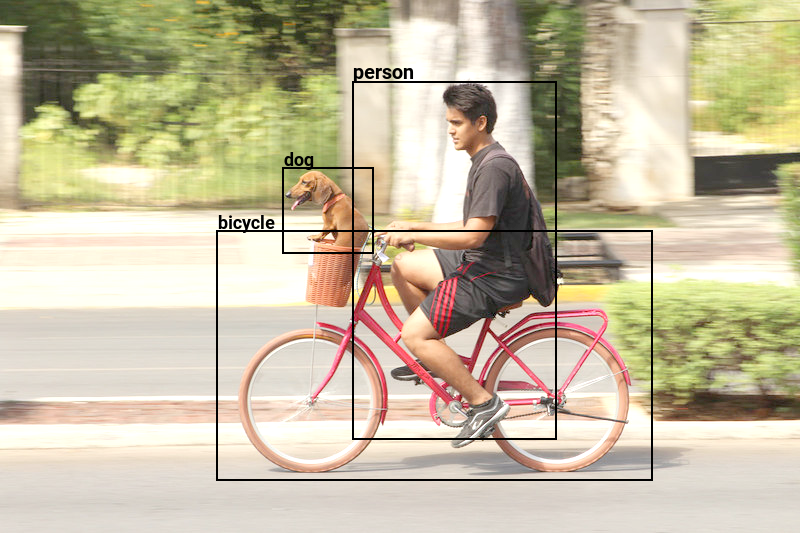
\includegraphics[width=\textwidth]{dogbike_annotated}
\centering
\caption{Visualization of the labels and bounding boxes emitted by YOLO when given an image depicting a cyclist with a dog.}
\end{figure}

YOLO is written in C, using the Darknet neural network library \citep{darknet13}.
It can be used in Python with the TensorFlow machine learning library and the Darkflow library which translates a Darknet model to TensorFlow.

When invoked from Python, the return value is a collection of dict objects, each containing a label, coordinates and a confidence score, as exemplified in \autoref{lst:yoloout}.
Results with confidence over a certain threshold are cast into \gls{ttr} records.
In this process, the bounding box coordinates are cast from a top-left and bottom-right tuple $\langle\langle x_1, y_1\rangle, \langle x_2, y_2\rangle\rangle$ to a center-width-height tuple $\langle x_c, y_c, w, h\rangle$ (later defined as the $Segment$ type), as the latter is more adequate for the spatial classification used in this project.

\begin{lstlisting}[label=lst:yoloout, caption=Example output of YOLO invocation]
[
    {
        'topleft': {'x': 354, 'y': 86},
        'bottomright': {'x': 551, 'y': 437},
        'label': 'person',
        'confidence': 0.80116189,
    },
    {
        'topleft': {'x': 224, 'y': 234},
        'bottomright': {'x': 646, 'y': 476},
        'label': 'bicycle',
        'confidence': 0.85828924,
    },
	...
]
\end{lstlisting}



\subsection{Objects and perception}

The perception of objects in this model is largely based on \cite{lspc}.
First, the object detection algorithm returns a set of \textit{perceptual objects}.
Each of them is evidence that a certain location is associated with a certain property (such as being a dog), but it does not constrain any individual to this association.
Second, an \textit{individuated object} is generated for each perceptual object.
This describes the situation that there is an individual, which has the given property, at the given location.
%In the \gls{ttr} implementation (presented in full in \autoref{sec:ttrmodel}), the individuated object is a type.
%[what's so good about it being a type?] \cite{BarwiseSituationsAttitudes1981}

In \cite{lspc}, the world has the form of a 3D point space rather than a 2D image.
This necessitates different types for the perceptual input and the locations of perceived objects.
In the point space case, the $PointMap$ set type is used for the full ``world'', and any part of the world is simply a subset of it, so it is also a $PointMap$.
In our case, $Image$ is used for the full image but we use $Segment$ to refer to parts of it.



\subsection{Spatial relations}
\label{sec:method-spatrel}
% Classification algorithm non-TTR. Simplistic, compare to sophisitcated alternatives.

Our method of spatial relation classification is inspired by \cite{ttrspat} but more simplistic.
One simplification is that the reference frame is fixed.
In the words of \cite{Garnhamunifiedtheorymeaning1989}, this means we only consider the deictic meaning of spatial relation terms, and not the intrinsic.
``Left'' will mean to the left in the plane of the image, even if the reference object is turned on the side or toward the viewer.
Another simplification is the neglection of the \textit{functional} aspects of spatial relations \citep{CoventryInterplayGeometryFunction2001}.

In our model, a spatial classifier $\kappa$ takes two locations and returns a boolean result.
We have implemented spatial classifiers as Python functions.
For the purpose of this thesis, no sophisticated spatial classification has been considered.
Instead, a naive comparison between centers of bounding boxes was implemented.
This was done for the four relations ``left'', ``right'', ``above'' and ``below''.



\subsection{Language and \acrfull{vqa}}
\label{sec:languagevqa}

In contrast to full \gls{vqa} systems, the model presented in this thesis will be restricted to a limited type of questions, namely polar questions on the location of one object in relation to another.
Such a question has a corresponding declarative statement:
The question ``Can you see them?'' corresponds to the statement ``You can see them''.
[TODO source?]

[TODO check \cite{RooyPolarQuestions2003}, (sources of) \cite{AloniQuantificationConceptualCovers2001}]

Giving the natural-language utterance a representation in the same formal framework as the image allows comparing them to each other.
% TODO Comparing?
The system will laborate with a \textit{question type} ($Q$) representing the question, as well as a \textit{scene type} ($S$) representing the perceived scene.

The situation described by the question type will be true if there exists a witness of that type, $r:Q$ \citep{BarwiseSituationsAttitudes1981,CooperAustiniantruthattitudes2005}.
The scene type, on the other hand, is considered true by virtue of being generated by perceptual classification.
It follows that the question type is true if it is a supertype of the scene type.
Thus, rather than looking for a witness to the question type, we formulate the problem as subtype checking, described in detail in \autoref{sec:subtyperelabeling}.
%However, the subtype relation requires matching field labels, which will not be the case here, as labels are generated on the fly.
%Thus, the condition is reformulated to allow relabeling \citep[pp. 133–135]{CooperTypetheorylanguage2016}:
The question is answered with ``yes'' or ``no'' depending on whether the scene type is a subtype of the question type, $S \sqsubseteq Q$.

The existing research on \gls{ttr}-based approaches to natural-language parsing, overviewed in \autoref{sec:ttnlp}, might be extensive enough to cover the kind of utterances considered here.
However, there is currently no implementation available and ready to use, and parsing is not within the main focus of this thesis.
Therefore, the natural-language parsing implemented for this thesis is instead a simplistic one, detailed in \autoref{sec:parsing}
%It uses feature structure context-free grammar (FCFG) tools available in NLTK \citep{BirdNaturalLanguageProcessing2009} to parse text into \gls{fol} expressions.
%With a custom function, the \gls{fol} expressions are transformed to a TTR record type.
%As an example, the question ``Is there a dog to the left of a car?'' is parsed into the type in \autoref{eq:uttex}.

%\begin{equation}\label{eq:uttex}
%\left[\begin{array}{rcl}
%\text{x} &:& Ind\\
%\text{y} &:& Ind\\
%\text{c}_\text{dog} &:& \text{dog}(x)\\
%\text{c}_\text{car} &:& \text{car}(y)\\
%\text{c}_\text{left} &:& \text{left}(x, y)\\
%\end{array}\right]\end{equation}

%[classification before/after question]


\section{Results}
\label{sec:results}

In this section, the \gls{ttr} model is formally defined, and some snippets of crucial Python code are presented.
The implementation necessitated some extensions to PyTTR which are also presented.
[The vqa application is presented? sd]



\subsection{\Gls{ttr} model}

Three basic types exist in the model.

\begin{description}
\item [$Ind$] A single individual object (or person), such as the reader or the Eiffel Tower.
\item [$Int$] An integer, such as 415.
\item [$Image$] A 2-dimensional digital image. It serves as an identifier to a set of extracted information, and its file type and actual data is not important in this thesis.
\end{description}

A $Segment$ is a record type describing a rectangular bounding box within an (implicit) image (\autoref{eq:seg}).
Its fields contain the center coordinates of the box ($cx$ and $cy$) and the width ($w$) and height ($h$) of the box.
$Ppty$ is the type of functions that can be applied to an individual and return a type (\autoref{eq:ppty}).
In our account the resulting type will be restricted to a ptype that is dependent on the individual, thus describing a property of it.

\begin{equation}\label{eq:seg}
Segment = \left[\begin{array}{rcl}
\text{cx} &:& Int\\
\text{cy} &:& Int\\
\text{w} &:& Int\\
\text{h} &:& Int
\end{array}\right]\end{equation}

\begin{equation}\label{eq:ppty}
Ppty = (Ind \rightarrow Type)\end{equation}

A perceptual object is a record of the type $Obj$ (\autoref{eq:obj}).
An example record is given in \autoref{eq:objrec}.
%$Obj$ records are the result of performing \textit{object detection}.
%This fact is expressed in TTR as the function type $ObjDetector$ (\autoref{eq:objdetector}).
An object detector is a function from an image to a set of perceptual objects, as captured by the $ObjDetector$ function type (\autoref{eq:objdetector}).

\begin{equation}\label{eq:obj}
Obj = \left[\begin{array}{rcl}
\text{seg} &:& Segment\\
\text{pfun} &:& Ppty \\
\end{array}\right]\end{equation}

\begin{equation}\label{eq:objrec}
obj =
\left[\begin{array}{rcl}
\text{seg} &=& \left[\begin{array}{rcl}
\text{cx} &=& 138\\
\text{w} &=& 276\\
\text{cy} &=& 654\\
\text{h} &=& 809
\end{array}\right]\\
\text{pfun} &=& \lambda v:Ind\ .\ \text{person}(v)\\
\end{array}\right] : Obj\end{equation}

\begin{equation}\label{eq:objdetector}
ObjDetector = ( Image \rightarrow [Obj] )
\end{equation}



\subsubsection{Individuation}

Moving from the perceptual to the conceptual domain, an individuated object is expressed not as a record, but as a record type.
The individuated object record type is a subtype of $IndObj$ (\autoref{eq:indobj}).
Here, $x$ is an individual and $loc$ is a location.
$cl$ specifies that $loc$ is the location of $x$, and the purpose of $cp$ is to declare a property of $x$.
$PTy$ is defined as a supertype of all ptypes (\autoref{eq:pty}).

\begin{equation}\label{eq:indobj}
IndObj = \left[\begin{array}{rcl}
\text{x} &:& Ind \\
\text{loc} &:& Segment \\
\text{cp} &:& PTy \\
\text{cl} &:& \text{location}(\text{x}, \text{loc}) \\
\end{array}\right]
\end{equation}

\begin{equation}\label{eq:pty}
PTy : Type
\end{equation}

A function for generating an $IndObj$ subtype from an $Obj$ record is known from \cite{lspc} as an \textit{individuation function}.
It is typed as $IndFun$ (\autoref{eq:indfun}).

\begin{equation}\label{eq:indfun}
IndFun = ( Obj \rightarrow RecType )
\end{equation}

The record type resulting from applying an $IndFun$ function should be a subtype of $IndObj$.

For each record type returned by the individuation function, a record is simultaneously created.
The $loc$ value of this record is naturally identical to the $seg$ value of the $Obj$ input record.
Objects for the remaining fields need to be instantiated on the spot.
Object creation is notated here as $A_{new}$, where the symbol $A$ may vary for the sake of readability.
%For the $x$ field, we create a new individual object $a_{new} : Ind$.
%For the ptype fields $cp$ and $cl$, we also create new objects $e_{new} : r.\text{pfun}(\text{x})$ and $e_{new} : \text{location}(\text{x}, \text{loc})$.

The individuation function is defined in \autoref{eq:indfundef}, with an example application in \autoref{eq:indfunrec}.
The definition uses manifest fields to denote the \textit{fully specified} record type, or singleton record type.

\begin{equation}\label{eq:indfundef}
Individuate = \lambda r : Obj\ . \left[\begin{array}{lcl}
    \text{x} = a_{new} &:& Ind \\
    \text{cp} = e_{new} &:& r.\text{pfun}(\text{x}) \\
    \text{cl} = e_{new} &:& \text{location}(\text{x}, \text{loc}) \\
    \text{loc} = r.\text{seg} &:& Segment\\
\end{array}\right]
\end{equation}

\begin{equation}\label{eq:indfunrec}
Individuate(
\left[\begin{array}{rcl}
\text{seg} &=& \left[\begin{array}{rcl}
\text{cx} &=& 138\\
\text{w} &=& 276\\
\text{cy} &=& 654\\
\text{h} &=& 809
\end{array}\right]\\
\text{pfun} &=& \lambda v:Ind\ .\ \text{person}(v)\\
\end{array}\right]
) =
\left[\begin{array}{lcl}
    \text{x} = a_0 &:& Ind \\
    \text{cp} = e_0 &:& \text{person}(\text{x}) \\
    \text{cl} = e_1 &:& \text{location}(\text{x}, \text{loc}) \\
    \text{loc} = \left[\begin{array}{rcl}
\text{cx} &=& 138\\
\text{w} &=& 276\\
\text{cy} &=& 654\\
\text{h} &=& 809
\end{array}\right] &:& Segment\\
\end{array}\right]
\end{equation}



\subsubsection{Spatial relations}

Relations may hold between pairs of individuated objects.
How do we detect and model a certain relation between such a pair?

Since we are interested in the spatial relation between a \textit{reference object} and a \textit{located object}, we will be constructing tuple-like records of the type $LocTup$ defined in \autoref{eq:loctup}.
Records of this type contain instantiations (records) of two $IndObj$ record types.
In \autoref{eq:clf}, a classifier is modeled as a function from such a record to a new record type which should describe the relation.

\begin{equation}\label{eq:loctup}
LocTup = \left[\begin{array}{rcl}
    \text{lo} &:& IndObj \\
    \text{refo} &:& IndObj \\
    \end{array}\right]
\end{equation}

\begin{equation}\label{eq:clf}
ClfFun = ( LocTup \rightarrow RecType )
\end{equation}

For instance, a classifier for ``left'' might look like in \autoref{eq:leftclfdef}, where $\kappa_{left}$ is a non-TTR, boolean function.
Of course, the requirement that the individual $r.\text{lo}.\text{x}$ is actually located at $r.\text{lo}.\text{loc}$ (and same for $r.\text{refo}$) is implicit from the typing as $IndObj$, where the field $\text{cl} : \text{location}(\text{x}, \text{loc})$ is necessarily present.

\begin{equation}\label{eq:leftclfdef}
\lambda r : LocTup \ .\ 
\begin{cases}
\left[\begin{array}{rcl}
    \text{cr} &:& \text{left}(r.\text{lo}.\text{x}, r.\text{refo}.\text{x}) \\
\end{array}\right],
& \text{if } \kappa_{left}(r.\text{lo}.\text{loc}, r.\text{refo}.\text{loc}) \\
[], & \text{otherwise}
\end{cases}
\end{equation}



\subsubsection{Agent}

Now, the perceptual-conceptual pieces described above are combined.
We are building an agent who receives classified and located objects of an image, apprehends their basic status and spatial relations, and answers natural-language questions about the image.

\begin{equation}\label{eq:agent}
Agent = \left[\begin{array}{rcl}
    \text{objdetector} &:& ObjDetector \\
    \text{indfun} &:& IndFun \\
    \text{appr} &:& [(Rec \rightarrow RecType)] \\
    \text{state} &:& AgentState \\
    \end{array}\right]
\end{equation}

\begin{equation}\label{eq:state}
AgentState = \left[\begin{array}{rcl}
    \text{img} &:& Image \\
    \text{perc} &:& [Obj] \\
    \text{bel} &:& [RecType] \\
    \text{utt} &:& RecType \\
    \end{array}\right]
\end{equation}

The fields $objdetector$, $indfun$ and $appr$ of $Agent$ are to be statically defined for a specific agent.
While running, the agent will modify the $AgentState$ record in $state$.

\begin{enumerate}
\item Visual input in the form of an image is received and assigned to $agt.\text{state}.\text{img}$.
\item $objdetector$ is invoked on $agt.\text{state.img}$ and creates a collection of records that are assigned to $agt.\text{state}.\text{perc}$.
\item $indfun$ is, in turn, invoked on each record in $agt.\text{state.perc}$ and resulting record types are added to $agt.\text{state.bel}$.
\item Now, each function in $agt.\text{appr}$ are applied:
	\begin{enumerate}
	\item The fields of the domain record type of the function is considered its arguments.
	\item Each combination of $agt.\text{state.bel}$ record types that matches the argument types is considered for input.
	\item A record is instantiated for each input record type, and the records are combined into one that matches the domain record type of the function.
	\item Resulting record types are added to $agt.\text{state.bel}$
	\end{enumerate}
	For example, the \textit{left} classifier in \autoref{eq:leftclfdef} is applied to each pair of $IndObj$ after instantiating and combining records into a $LocTup$.
\item Any language input is parsed and the resulting record type assigned to $agt.\text{state.utt}$.
\item The record types in $agt.\text{state.bel}$ are combined/concatenated. If the resulting record type is a relabel-subtype of $agt.\text{state.utt}$, a positive answer is emitted; otherwise a negative answer is emitted.
\end{enumerate}

An example state of an agent $agt$ is shown in \autoref{eq:agt}.

\begin{landscape}
\begin{equation}\label{eq:agt}
\renewcommand{\arraystretch}{1.2}
agt = \left[\begin{array}{rcl}
    \text{objdetector} &=& \mathtt{yolo\_detector} \\
    \text{indfun} &=& \mathtt{individualize} \\
    \text{appr} &=& [Clf_{left}, Clf_{right}, Clf_{above}, Clf_{below}] \\
    \text{state} &=& \left[\begin{array}{rcl}
		\text{img} &=& \mathtt{dogride.jpg} \\
		\text{perc} &=& [
			\left[\begin{array}{rcl}
				\text{seg} &=& \left[\begin{array}{rcl}
					\text{w} &=& 197\\
					\text{cx} &=& 452\\
					\text{h} &=& 351\\
					\text{cy} &=& 261
					\end{array}\right]\\
				\text{pfun} &=& \lambda a:Ind\ .\ \text{person}(a)
				\end{array}\right],
			\left[\begin{array}{rcl}
				\text{seg} &=& \left[\begin{array}{rcl}
					\text{w} &=& 422\\
					\text{cx} &=& 435\\
					\text{h} &=& 242\\
					\text{cy} &=& 355
					\end{array}\right]\\
				\text{pfun} &=& \lambda a:Ind\ .\ \text{bicycle}(a)
				\end{array}\right],
			...
			] \\
		\text{bel} &=& \begin{array}{l} [
			\left[\begin{array}{rcl}
				\text{x} = a_0 &:& Ind\\
				\text{cp} = e_0 &:& \text{person}(x)\\
				\text{cl} = e_{1} &:& \text{location}(x, loc)\\
				\text{loc} = \left[\begin{array}{rcl}
					\text{w} &=& 197\\
					\text{cx} &=& 452\\
					\text{h} &=& 351\\
					\text{cy} &=& 261
					\end{array}\right]
					&:& Segment \\
				\end{array}\right],
			{}{} \left[\begin{array}{rcl}
				\text{cr}=e_6 &:& \text{above}(a_{0}, a_{1})
				\end{array}\right],
			... ]
			\end{array} \\
		\text{utt} &=& \left[\begin{array}{rcl}
			\text{x} &:& Ind\\
			\text{y} &:& Ind\\
			\text{c}_\text{0} &:& \text{dog}(x)\\
			\text{c}_\text{1} &:& \text{bicycle}(y)\\
			\text{c}_\text{2} &:& \text{left}(x, y)\\
			\end{array}\right] \\
		\end{array}\right] \\
    \end{array}\right]
\end{equation}
\end{landscape}



\subsection{Python implementation}

The full code is published as a Jupyter Notebook \footnote{\url{https://github.com/arildm/imagettr}}.

\subsubsection{Utility functions}

These are PyTTR-related functions that are used in later code.

\begin{lstlisting}[label=lst:utility,caption=Utility functions]
from functools import reduce

# The Ind TTR type is used by these utility functions so it needs defining here already.
Ind = BType('Ind')
    
def copy_rectype(T):
    """Make another copy of a record type."""
    R = RecType()
    for k, v in T.comps.__dict__.items():
        R.addfield(k, v)
    return R

def rectype_relabels(T, rlbs):
    """Relabel multiple fields, given a dict of from-to pairs."""
    for k1, k2 in rlbs.items():
        T.Relabel(k1, k2)
    return T

def rectype_merges(Ts):
    """Merge a list of RecTypes."""
    return reduce((lambda T, U: T.merge(U)), Ts, RecType())

def is_basic_type(T):
    """Whether a type is a "basic field", i.e. a BType or a SingletonType of a BType."""
    tn = lambda T: type(T).__name__
    return (tn(T) == 'BType') if tn(T) != 'SingletonType' else is_basic_type(T.comps.base_type)

def basic_fields(T):
    """The labels of basic fields in a RecType."""
    return [k for k, v in T.comps.__dict__.items() if is_basic_type(v)]

def nonbasic_fields(T):
    """The labels of non-basic fields in a RecType."""
    return [k for k, v in T.comps.__dict__.items() if not is_basic_type(v)]

ptypes = dict()
def mkptype(sym, types=[Ind], vars=['v']):
    """Make preds and ptypes identifiable by their predicate names."""
    id = '/'.join([sym, ','.join(show(type) for type in types), ','.join(vars)])
    if id not in ptypes:
        ptypes[id] = PType(Pred(sym, types), vars)
    return ptypes[id]

def create_fun(pred_name, vars=['a']):
    """Create a function of a given number of Inds (length of vars).
    
    Example: create_fun('give', 'abc') --> \a. \b. \c. give(a, b, c)
    """
    fun = mkptype(pred_name, types=[Ind]*len(vars), vars=vars)
    for v in reversed(vars):
        fun = Fun(v, Ind, fun)
    return fun
\end{lstlisting}

\subsubsection{Necessary extensions to PyTTR}

\begin{lstlisting}[label={lst:mergeunconflict},caption={merge\_unconflict()}]
def unique_labels(T):
    """Relabel a RecType so each field label is unique over all RecTypes."""
    for l, v in T.comps.__dict__.items():
        if '_' not in l:
            T.Relabel(l, gensym(l))
    return T

def merge_unconflict(T1, T2):
    """Merge two RecTypes after making sure they do not share any field labels."""
    T1c = unique_labels(copy_rectype(T1))
    T2c = unique_labels(copy_rectype(T2))
    return T1c.merge(T2c)
\end{lstlisting}

For example, if $T_1 = [x:Ind]$ and $T_2 = [x:Ind]$, then $\mathtt{merge\_unconflict}(T_1, T_2)$ evaluates to $\left[\begin{array}{rcl} x_0&:&Ind \\ x_1&:&Ind \end{array}\right]$ (or a similar record type with different subscript indices).

\begin{lstlisting}[label={lst:useindfieldlabels},caption={use\_ind\_field\_labels()}]
def use_ind_field_labels(T):
    """c:foo(a) becomes c:foo(x) if x=a:Ind is present."""
    T = copy_rectype(T)
    for l, v in T.comps.__dict__.items():
        if isinstance(v, SingletonType) and v.comps.base_type == Ind:
            a = v.comps.obj
            T.Relabel(a, l)
            # Undo the relabeling of the Ind field itself.
            T.comps.__dict__[l] = SingletonType(Ind, a)
    return T
\end{lstlisting}

\begin{lstlisting}[label={lst:unsingleton},caption={unsingleton()}]
def unsingleton(T):
    """Remove singleton specifications of a type: x=a:Ind becomes x:Ind."""
    T2 = RecType()
    for l, v in T.comps.__dict__.items():
        T2.addfield(l, v if not isinstance(v, SingletonType) else v.comps.base_type)
    return T2
\end{lstlisting}

\subsubsection{YOLO}

\begin{lstlisting}[label=lst:yolo, caption=Invoking YOLO]
from darkflow.net.build import TFNet
import numpy as np

tfnet = TFNet({"model": "yolo/yolo.cfg", "load": "yolo/yolo.weights",
    'config': 'yolo', "threshold": 0.2})

yolo_out = dict()
def yolo(img):
    """Invokes YOLO on a PIL image, caches and returns the result."""
    if str(img) not in yolo_out:
        yolo_out[str(img)] = tfnet.return_predict(np.array(img))
    return yolo_out[str(img)]
\end{lstlisting}

\subsubsection{PyTTR implementation}

The basic type $Ind$ was defined along with the utility functions in \autoref{lst:utility}.

\begin{lstlisting}[label={lst:pyttrbasic},caption={individuate()}]
Int = BType('Int')
Int.learn_witness_condition(lambda x: isinstance(x, int))

Image = BType('Image')
Image.learn_witness_condition(lambda x: isinstance(x, PIL.Image.Image))

Segment = RecType({'cx': Int, 'cy': Int, 'w': Int, 'h': Int})
Ppty = FunType(Ind, Ty)
Obj = RecType({'seg': Segment, 'pfun': Ppty})

Objs = ListType(Obj)
ObjDetector = FunType(Image, Objs)
\end{lstlisting}

[something about the object detector]

\begin{lstlisting}[label=lst:pyttr_yolo, caption=Connecting YOLO output to PyTTR]
def yolo_coords(o):
    """Extract the coordinates from a YOLO output item as ((x0,y0), (x1,y1))."""
    return (o['topleft']['x'], o['topleft']['y']), (o['bottomright']['x'], o['bottomright']['y'])

def xy1xy2_to_cwh(x1, y1, x2, y2):
    '''Transform to center, width and height.'''
    return {'cx': int(x1/2 + x2/2), 'cy': int(y1/2 + y2/2), 'w': x2 - x1, 'h': y2 - y1}

def yolo_detector(i):
    """Creates IndObj records for YOLO results."""
    return [Rec({
        'seg': Rec(xy1xy2_to_cwh(*yolo_coords(o)[0], *yolo_coords(o)[1])),
        'pfun': create_fun(o['label'].replace(' ', '_')),
    }) for o in yolo(i)] # @todo RBG/BGR?
ObjDetector.witness_cache.append(yolo_detector)

objs = yolo_detector(img)
\end{lstlisting}

PyTTR includes a class $Fun$ which models TTR functions.
It does not, however, support usage of the argument within the function body.
The individuation function was therefore implemented in Python.

\begin{lstlisting}[label={lst:individuate},caption={individuate()}]
PTy = Type('PTy')
PTy.learn_witness_condition(lambda p: isinstance(p, HypObj) \
    and forsome(p.types, lambda t: isinstance(t, PType)))

IndObj = RecType({
    'x' : Ind,
    'loc' : Segment,
    'cp' : PTy,
    'cl' : create_fun('location', 'ab').app('x').app('loc'),
})
IndFun = FunType(Obj, RecTy)

def individuate(r):
    cp = r.pfun.app('x')
    cl = create_fun('location', 'ab').app('x').app('loc')
    return RecType({
        'x': SingletonType(Ind, Ind.create()),
        'cp': SingletonType(cp, cp.create()),
        'loc': SingletonType(Segment, r.seg),
        'cl': SingletonType(cl, cl.create()),
    })
IndFun.witness_cache.append(individuate)

indobjs = [individuate(r) for r in objs]
\end{lstlisting}

[something about spatial relation classifiers]

\begin{lstlisting}[label=lst:relclf, caption=Spatial relation classifiers]
from itertools import product

LocTup = RecType({'lo': IndObj, 'refo': IndObj})
ClfRes = RecType({'cr': PTy})
RelClf = FunType(LocTup, ClfRes)

location_relation_classifiers = {
    'left': lambda a, b: a.cx < b.cx,
    'right': lambda a, b: a.cx > b.cx,
    'above': lambda a, b: a.cy < b.cy,
    'below': lambda a, b: a.cy > b.cy,
}

def get_relclfs():
    for pred, f in location_relation_classifiers.items():
        def relclf(r):
            if f(r.lo.loc, r.refo.loc):
                c = create_fun(pred, 'ab').app(r.lo.x).app(r.refo.x)
                return RecType({'cr': SingletonType(c, c.create())})
            return RecType()
        RelClf.witness_cache.append(relclf)
        yield relclf

def find_all_rels(indobjs):
    """Find all relations between IndObj records."""
    for relclf in get_relclfs():
        for loT, refoT in product(indobjs, indobjs):
            loctup = Rec({'lo': loT.create(), 'refo': refoT.create()})
            yield relclf(loctup)

rels = list(find_all_rels(indobjs))
\end{lstlisting}

\begin{lstlisting}[label=lst:bel, caption=Combining beliefs.]
def combine_beliefs(bel):
    """Combine a list of belief record types into one."""
    return unsingleton(use_ind_field_labels(reduce(merge_unconflict, bel, RecType())))

bel = indobjs + rels
bel_comb = combine_beliefs(bel)
\end{lstlisting}

[...]
 Parsing to PyTTR cannot really be done directly. NLTK feature grammars support strings and FOPC. Variable substitution is only allowed in FOPC. We produce a FOPC conjunction of ptypes, for each of which we create a new field.

\begin{lstlisting}[label=lst:grammar, caption=Basic parsing of natural language into PyTTR object.]
import nltk

grammar = nltk.grammar.FeatureGrammar.fromstring(r'''
%start S
S[SEM=<?s(x) & ?vp(x, y)>] -> NP[SEM=?s] VP[SEM=?vp]
NP[SEM=<?det(?n)>] -> Det[SEM=?det] N[SEM=?n]
Det[SEM=<\P a.P(a)>] -> 'a' | 'an'
N[SEM=<dog>] -> 'dog'
N[SEM=<car>] -> 'car'
N[SEM=<person>] -> 'person'
N[SEM=<bicycle>] -> 'bicycle'
N[SEM=<backpack>] -> 'backpack'
VP[SEM=?pp] -> 'is' PP[SEM=?pp]
PP[SEM=<\a b.(?prep(a, b) & ?o(b))>] -> Prep[SEM=?prep] NP[SEM=?o]
Prep[SEM=<left>] -> 'to' 'the' 'left' 'of'
Prep[SEM=<right>] -> 'to' 'the' 'right' 'of'
Prep[SEM=<above>] -> 'above'
Prep[SEM=<under>] -> 'under'
''')
parser = nltk.FeatureChartParser(grammar)

def fopc_to_pyttr(expr, T=RecType()):
    """Turns a FOPC object into a RecType."""
    from nltk.sem.logic import ApplicationExpression, AndExpression
    if isinstance(expr, ApplicationExpression):
        pred, args = expr.uncurry()
        T.addfield(gensym('c'), mkptype(str(pred), vars=[str(a) for a in args]))
        for x in args:
            if str(x) not in T.comps.__dict__:
                T.addfield(str(x), Ind)
    if isinstance(expr, AndExpression):
        fopc_to_pyttr(expr.first, T)
        fopc_to_pyttr(expr.second, T)
    return T

def eng_to_pyttr(text):
    trees = parser.parse(text.lower().split())
    sem = nltk.sem.root_semrep(list(trees)[0])
    T = fopc_to_pyttr(sem)
    return T
\end{lstlisting}

[...]

\begin{lstlisting}[label=lst:subtyperlb, caption=Implementation of the relabel-subtype relation.]
from itertools import permutations, combinations

def find_subtype_relabeling(T, U):
    '''Could record type T be a sub type of record type U if relabeling in T is allowed?'''
    # Find possible relabelings for basic-type fields
    basic_label_permutations = set(ps[:len(basic_fields(U))] for ps in permutations(basic_fields(T)))
    
    for tks in basic_label_permutations:
        # Copy U and try a basic-fields relabeling
        U2 = copy_rectype(U)
        rlb = dict(zip(basic_fields(U), tks))
        rectype_relabels(U2, rlb)
        
        # For each U field, find a T field that is a subtype
        match = dict()
        for uk in nonbasic_fields(U2):
            for tk in nonbasic_fields(T):
                if T.comps.__dict__[tk].subtype_of(U2.comps.__dict__[uk]):
                    match[uk] = tk
                    break
            if uk not in match:
                break

        # Successful if all non-basic fields match.
        if len(match) == len(nonbasic_fields(U2)):
            return dict(**rlb, **match)
    return None
\end{lstlisting}

\begin{lstlisting}
def validate_utt(utt, bel):
    return bool(find_subtype_relabeling(combine_beliefs(bel), utt))

def relabel_utt(utt, bel_comb):
    """Relabels an utterance record type to match the combined beliefs.
    
    The result will be a subtype of bel_comb.
    """
    rlb = find_subtype_relabeling(bel_comb, utt)
    return rectype_relabels(utt, rlb)
\end{lstlisting}

\subsection{Discussion}
\label{sec:discussion}

Contradiction of Logan \& Sadler's "evidence" for their "theory of apprehension" (which is different from mine)? (Already Regier \& Carlson did.)

Not a full VQA solution.
It can only answer one question type, and only in the form "A P is R a Q", which is not even a question.
With only the extension of parsing, it could understand (= educe situation record types) more complex forms like "A R1 B1 and R2 B2", "A1 R1 B1 and A2 R2 B2".
"What is R B?"
"What color is the A?"
"How many A are there?" etc.

...

PyTTR extensions (here or Conclusions?)

Functional aspect (Coventry).


\section{Discussion}
\label{sec:discussion}



\subsection{Model limitations}

As discussed in \autoref{sec:method-spatrel}, our treatment of spatial relations excludes the intrinsical meaning and functional aspects, in favor of model simplicity and easy implementation.
Both features are treated in terms of \gls{ttr} by \cite{ttrspat}.
The former requires a notion of the orientation of reference objects.
Assuming an object classifier with this capability were available, implementing intrinsical spatial relations would not be a large step from the present model.
Support for the functional aspect of spatial relations requires two things.
Firstly, classifiers for functional relations (such as $\text{protects(o}_3\text{.a, o}_1\text{.a, o}_2\text{.a)}$ in \cite{ttrspat}, for an umbrella protecting a man from rain).
Secondly, prediction from a set of functional relations to spatial classifiers that are sensitive to those functional relations.
The second is needed to activate the appropriate spatial relation term depending on which functional relations are true according to the classifiers in the first.

The model is restricted to a limited type of polar questions, far from the range of question types in the \gls{vqa} dataset \citep{AgrawalVQAVisualQuestion2015}.
Vast extensions to the language parsing, the perceptual classification and the comparation of question and scene are possible and required in order to answer more advanced questions.
Some examples are:
further property classification (``Is the dog brown?''),
wh-questions (``What is to the left of the car?''),
quantities (``How many flowers are there?''),
inference (``Does this person have 20/20 vision?'', for an image where a person is wearing glasses).



\subsection{TTR coverage}



\subsection{VQA performance}



\subsection{Comparison to different approaches}
% a) VQA models, b) other perception/language models





\section{Conclusions}
\label{sec:conclusions}
\glsresetall

Within this project, the foundations of \gls{vqa} have been implemented in \gls{ttr}.
The result is an executable application powered by PyTTR.

The formal-semantic framework behind the application provides transparency and reversibility, and enables relatively simple implementation of operations (such as verifying a proposition).
\Gls{ttr} is the single framework that serves to operate all parts of the pipeline: perception, language and grounding.

The model is one of few applications of the recently developed PyTTR library, which allows \gls{ttr} to be used in executable programs.
Extensions to PyTTR were made where needed.



\subsection{Future work}

Spatial classification and language parsing were achieved using minimal and simplistic implementations.
Substituting them with sophisticated systems would make for wider question coverage and higher question answering scores.
For instance, \cite{LoganComputationalAnalysisApprehension1996} proposes spatial templates, regions of acceptability and compound relations (like ``above to the right of'').

As discussed in \autoref{sec:method-spatrel}, the present treatment of spatial relations excludes the intrinsical meaning and functional aspects, in favor of model simplicity and easy implementation.
Both features are treated in terms of \gls{ttr} by \cite{ttrspat}.
The former requires a notion of the orientation of reference objects.
Assuming an object classifier with this capability were available, implementing intrinsical spatial relations would not be a large step from the present model.
Such a classifier might detect that a car is facing left in the image;
an object to the right in the image could then be classified as being ``behind'' the car.
Support for the functional aspect of spatial relations requires two things.
Firstly, classifiers for functional relations (such as $\text{protects}(o_3\text{.a}, o_1\text{.a}, o_2\text{.a})$ in \cite{ttrspat}, for an umbrella protecting a man from rain).
% TODO Be more clear below?
Secondly, prediction from a set of functional relations to spatial classifiers that are sensitive to those functional relations.
The second is needed to activate the appropriate spatial relation term depending on which functional relations are true according to the classifiers in the first.
That is, if the relation between the umbrella and the man is classified as ``protects'', then the spatial classifier selected for ``over'' should be one that includes this condition.

Extending the language domain should be an interesting topic for further research.
Keeping within the problem domain of geometric spatial relations, allowing other question types than polar questions is one direction to explore.
\citet[p. 156]{DobnikTeachingmobilerobots2009} lists four basic question types:
``Where is the chair?'',
``Is the table to the left of the chair?'' (this is the focus of this project),
``What is to the left of the chair?'' and
``What is the chair to the left of?''
Another is to widen the problem domain and add more properties and relations than a primary object class (``car'') and spatial relations.
For instance, attribute classifiers could recognise color, size, facial expressions and actions, in order to authorise questions such as ``Is the girl sitting down?'' and ``Where is the red flower?''.
Non-spatial relation classifiers could identify relations such as ``riding'' and ``talking to''.

The use of formal frameworks for question-answering tasks especially invites techniques for inference.
Consider an image of a person wearing glasses, and the question ``Does this person have 20/20 vision?''
It is reasonable to assume that a person is wearing glasses because they do not have perfect eyesight, to which ``20/20 vision'' is synonymous.
Inference could help to achieve the synonymity as well as the relationship between eyesight and wearing glasses.

%(b) left for future work in terms of (1) semantic representations of grounded language in TTR; (ii) their implementation in pyTTR; (iii) in the domain of visual question answering? 

%Classification after Q.


%\input{pyttr-output.tex}

\bibliography{imagettr}
\end{document}
